\documentclass[tikz]{standalone} 
\usetikzlibrary{decorations.pathmorphing,patterns}
%\renewcommand\familydefault{\sfdefault}

\usetikzlibrary{patterns}

\begin{document}
	
	%\tdplotsetmaincoords{0}{0}
	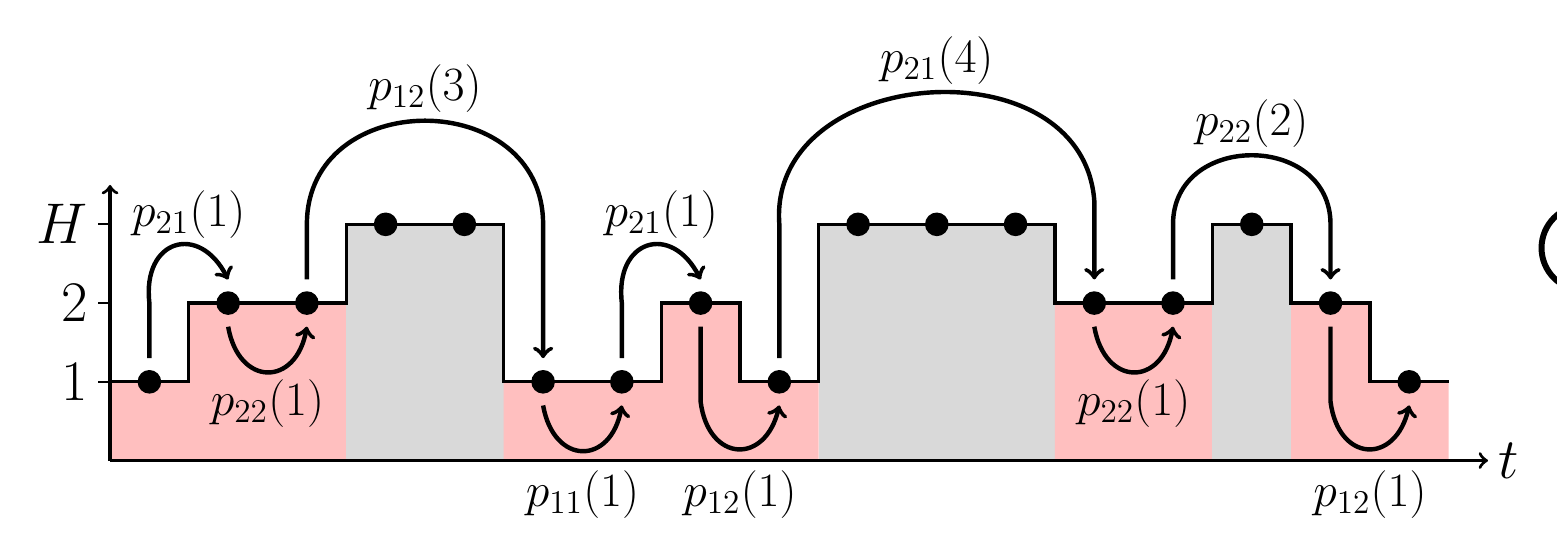
\begin{tikzpicture}
		\fill[red!25] (0,0) to (0,1) to (1,1) to (1,2) to (3,2) to (3,0);
		\fill[gray!30] (3,0) to (3,3) to (5,3) to (5,0);
		\fill[red!25] (5,0) to (5,1) to (7,1) to (7,2) to (8,2) to (8,1) to (9,1) to (9,0);
		\fill[gray!30] (9,0) to (9,3) to (12,3) to (12,0);
		\fill[red!25] (12,0) to (12,2) to (13,2) to (14,2) to (14,0);
		\fill[gray!30] (14,0) to (14,3) to (15,3) to (15,0);
		\fill[red!25] (15,0) to (15,2) to (16,2) to (16,1) to (17,1) to (17,0);
		\draw[thick] (-0.15 ,1)node[left]{\huge $1$} to (0,1);
		\draw[thick] (-0.15 ,2)node[left]{\huge $2$} to (0,2);
		\draw[thick] (-0.15 ,3)node[left]{\huge $H$} to (0,3);
		\draw[very thick] (0,1) to (1,1) to (1,2) to (3,2) to (3,3) to (4,3) to (4,3) to (5,3) to (5,1) to (7,1) to (7,2) to (8,2) to (8,1) to (9,1) to (9,3) to (11,3) to (11,3) to (12,3) to (12,3) to (12,2) to (13,2) to (14,2) to (14,3) to (15,3) to (15,2) to (16,2) to (16,1) to (17,1);
		\fill (0.5,1) circle (0.15);
		\fill (1.5,2) circle (0.15);
		\fill (2.5,2) circle (0.15);
		\fill (3.5,3) circle (0.15);
		\fill (4.5,3) circle (0.15);
		\fill (5.5,1) circle (0.15);
		\fill (6.5,1) circle (0.15);
		\fill (7.5,2) circle (0.15);
		\fill (8.5,1) circle (0.15);
		\fill (9.5,3) circle (0.15);
		\fill (10.5,3) circle (0.15);
		\fill (11.5,3) circle (0.15);
		\fill (12.5,2) circle (0.15);
		\fill (13.5,2) circle (0.15);
		\fill (14.5,3) circle (0.15);
		\fill (15.5,2) circle (0.15);
		\fill (16.5,1) circle (0.15);
		\draw[very thick,->] (0,0) to (17.5,0) node[right]{\huge $t$};
		\draw[very thick,->] (0,0) to (0,3.5);
		
		\draw[ultra thick, ->] (0.5,1.3) to (0.5,2) to [bend left=80, looseness=2] (1.5,2.3);
		\draw (1,2.7) node[above]{\LARGE $p_{21}(1)$};
		
		\draw[ultra thick, ->] (1.5,1.7) to [bend right=80, looseness=2] (2.5,1.7);
		\draw (2,1.15) node[below]{\LARGE $p_{22}(1)$};
		
		\draw[ultra thick, ->] (2.5,2.3) to (2.5,3) to [bend left=90, looseness=1.5] (5.5,3) to (5.5,1.3);
		\draw (4,4.3) node[above]{\LARGE $p_{12}(3)$};
		
		\draw[ultra thick, ->] (5.5,0.7) to [bend right=80, looseness=2] (6.5,0.7);
		\draw (6,0) node[below]{\LARGE $p_{11}(1)$};
		
		\draw[ultra thick, ->] (6.5,1.3) to (6.5,2) to [bend left=80, looseness=2] (7.5,2.3);
		\draw (7,2.7) node[above]{\LARGE $p_{21}(1)$};
		
		\draw[ultra thick, ->] (7.5,1.7) to (7.5,0.75) to [bend right=80, looseness=2] (8.5,0.7);
		\draw (8,0) node[below]{\LARGE $p_{12}(1)$};
		
		\draw[ultra thick, ->] (8.5,1.3) to (8.5,3) to [bend left=90, looseness=1.3] (12.5,3.3) to (12.5,2.3);
		\draw (10.5,4.65) node[above]{\LARGE $p_{21}(4)$};
		
		\draw[ultra thick, ->] (12.5,1.7) to [bend right=80, looseness=2] (13.5,1.7);
		\draw (13,1.15) node[below]{\LARGE $p_{22}(1)$};
		
		\draw[ultra thick, ->] (13.5,2.3) to (13.5,3) to [bend left=90, looseness=1.5] (15.5,3) to (15.5,2.3);
		\draw (14.5,3.85) node[above]{\LARGE $p_{22}(2)$};
		
		\draw[ultra thick, ->] (15.5,1.7) to (15.5,0.75) to [bend right=80, looseness=2] (16.5,0.7);
		\draw (16,0) node[below]{\LARGE $p_{12}(1)$};
		
		
		\begin{scope}[shift={(10.4,1.5)}]
			\scalebox{1.8}{
				\draw[very thick] (0,0) to (2,0);
				\draw[very thick] (0,0) to (1,-1.42);
				\draw[very thick] (2,0) to (1,-1.42);
				\draw[very thick,fill=white] (0,0) circle (0.3) node[]{$1$};
				\draw[very thick,fill = white] (2,0) circle (0.3) node[]{$2$};
				\draw[very thick,fill=white] (1,-1.42) circle (0.3) node[]{$H$};
			}
		\end{scope}
	\end{tikzpicture}
	
\end{document}